\documentclass{article}
\usepackage[utf8]{inputenc}
\usepackage[T1]{fontenc}
\usepackage[francais]{babel}
\usepackage{graphicx}     


% exemple papier seme https://hal.archives-ouvertes.fr/SEME
% https://hal.archives-ouvertes.fr/hal-01021660v1
% code GitHub : https://github.com/romainhild/pas


%TODO: ???
% entête: seme, dates, labo, lieu
% en bas de page logos (cnrs, amies)

% demander autorisation PAS pour utiliser images 
% marquer quelque part que l'on s'occuper que des conteneurs vides
% affiliations auteurs???
% mise en page, voir https://hal.archives-ouvertes.fr/hal-01021660v1 ???
% terminal sud du PAS

\title{SEME à Strasbourg\\ 
Approches mathématiques pour l'optimisation du placement des conteneurs dans la cour de stockage des terminaux portuaires du Port Autonome de Strasbourg}
\author{Beaude Laurence\footnote{Universit\'e C\^ote d'Azur, CNRS, INRIA COFFEE, 
	Laboratoire J.A. Dieudonn\'e, 
	Parc Valrose, 06108 Nice cedex 02, France.} 
\and 
Caldini-Queiros Céline\footnote{IRMA???}
\and 
Hild Romain
\and 
Maassarani Mohamad
\and 
Maumy-Bertrand Myriam
\and
Sala Lorenzo
}





\date{12-16 Novembre 2018}



%Sujet proposé par:
%logo pas ???


\begin{document}

\maketitle
\noindent
\textbf{Résumé :} le principe des Semaines d'\'Etude Mathématiques-Entreprises consiste à rassembler plusieurs jeunes chercheurs en mathématiques durant une semaine (du lundi au vendredi) autour de divers sujets proposés par des entreprises. 
Ce rapport détaille la réflexion d'une équipe, qui a eu lieu autour du sujet proposé par le Port Autonome de Strasbourg (abrégé en PAS). Suite à des travaux d'agrandissement dans le terminal à conteneurs Sud, le Port Autonome de Strasbourg se demande comment optimiser le placement des conteneurs dans leur cour de stockage. Nous considérons le problème de stockage des conteneurs vides car ces conteneurs sont nombreux et peuvent rester longtemps dans le terminal. Ainsi la surface occupée est conséquente et comme chaque déplacement de conteneur coûte cher, il est nécessaire d'optimiser le stockage pour réduire les kilomètres parcourus et les coûts d'exploitation. \\


\textbf{Mots clés :} Modélisation Mathématique, Stockage de conteneurs

\section{Introduction}

\subsection{Un peu d'histoire}

% citer papiers d'où on tire les infos (Myriam et https://www.researchgate.net/publication/294799315_Container_stacking_problem_a_survey)  ???

La conteneurisation doit son existence à Mc Lean qui a eu l'idée d'acheminer les marchandises dans des boîtes ou "conteneurs". En 1965, cette conteneurisation s'est développée sur l’Atlantique Nord puis s'est généralisée progressivement. Le conteneur est finalement devenu une boîte normée dont les standards ont été fixés en 1974 par l’ISO (International Standards Organisation). Cette période a aussi été marquée par l’apparition du transport multimodale qui consiste à utiliser plusieurs moyens de transport (bateau, train, camion) pour chaque marchandise. De nos jours, le transport fluvial et maritime des marchandises joue un rôle important dans un monde de plus en plus globalisé. Ainsi, depuis les dernières décennies, les plateformes d'échange multimodale, dont le Port Autonome de Strasbourg, doivent faire face à une augmentation de transbordement de conteneurs entre différents modes de transport. Cela pose le problème du stockage d'un nombre de plus en plus important de conteneurs dans les terminaux portuaires. En effet, lors de l'arrivée d'un conteneur, il est nécessaire de décider sa position exacte dans la cour de stockage en prenant en compte plusieurs contraintes tout en garantissant la sécurité du site. 


%



 %Dans ce cadre, les décisions qui doivent être prises peuvent être classées en trois catégories classiques : stratégiques, tactiques et opérationnelles. Au niveau stratégique, les décisions sur l’équipement à utiliser et son agencement sont prises. Au niveau tactique, il est nécessaire de définir le niveau de capacité d’équipements et d’effectifs, le placement des conteneurs, l’affectation de voies et aussi les horaires des bateaux et des trains. Le niveau opérationnel fait référence aux décisions opérationnelles quotidiennes. Eventuellement, au cours de ces opérations, plusieurs problématiques peuvent être potentiellement soulevées par les terminaux à conteneurs. En se basant sur les travaux de Steenken et al [Steenken 04], Stahlbock et Vob [Stahlbock 08] et Yuxuan [Yuxuan 05], les activités de base d’un terminal à conteneurs sont menées dans deux zones principales :
%– la zone à quai (quay zone) ;
%– la zone de cour (yard zone).






\subsection{Présentation du Port Autonome de Strasbourg}


Le Port Autonome de Strasbourg est une plateforme multimodale pour l'import/export d'une grande variété de produits. Il relie Strasbourg aux ports maritimes via le fleuve et le rail. En 2017, $420000$ équivalents vingt pieds (EVP) ont transité par le Port Autonome de Strasbourg et $30\%$ concerne l'Eurométropole. Le PAS exploite deux terminaux, dans cette étude nous nous focalisons sur le terminal Sud. Ce terminal transborde des conteneurs de 20 pieds ou de 40 pieds entre des barges et des camions, il n'y a pas de transport ferroviaire. Il possède deux portiques fluviaux à conteneurs dont l'un est mobile et l'autre permet de transporter des colis lourds (capacité $460$ tonnes).




\begin{figure}[!htb]
\centering
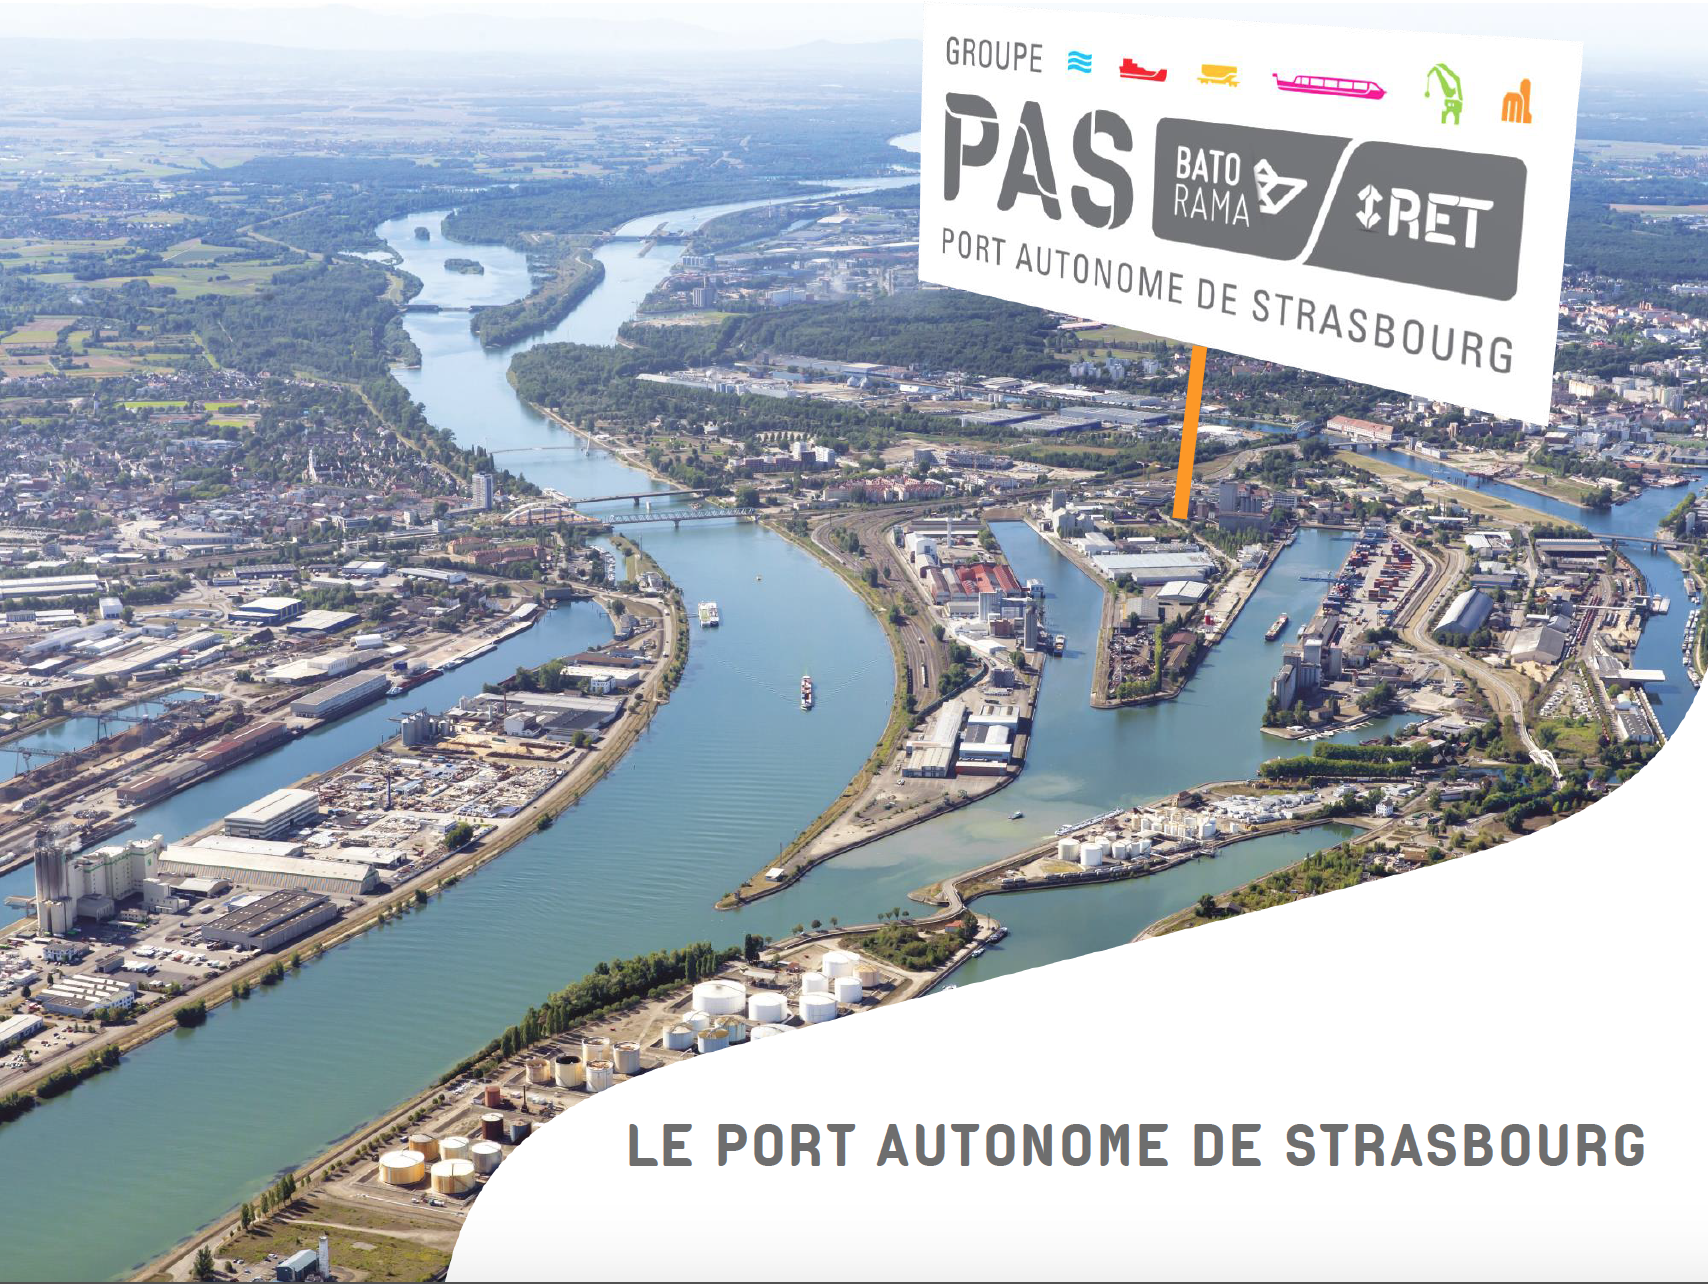
\includegraphics[width=0.7\linewidth]{images/PAS_satellite.png}
\caption{Vue du Terminal Nord du Port Autonome de Strasbourg.}
\label{fig:pas_satellite}
\end{figure}

\subsection{ ??? }

Cette note résume le travail réalisé pendant la Semaine d'\'Etude Mathématiques-Entreprises du 12 au 16 novembre 2018 à Strasbourg. 
Le port autonome de Strasbourg nous a soumis une question liée au stockage des conteneurs vides dans le port. 
Des travaux d'aménagement vont être réalisés et la question se pose de comment entreposer le plus efficacement les conteneurs vides dans la cour de stockage du PAS. 
En moyenne $3000$ conteneurs vides (toutes tailles confondues) sont sur le site avec $500$ entrées et $500$ sorties chaque jour, mais le port autonome n'a aucune visibilité sur la date de sortie d'un conteneur en particulier. 
Afin de ne pas facturer trop leur client, le port a généralement une politique de {\it First In, First Out} (abrégé en FIFO) pour qu'un conteneur en particulier ne reste pas trop longtemps entreposé. Pour respecter cette politique, les conteneurs sont stockés par bloc, un bloc contenant des conteneurs de mêmes dimensions (il existe trois tailles de conteneurs différents) et d'un même client (nous négligeons les trop petits clients).
Notre objectif est donc de proposer au port autonome de Strasbourg un plan de stockage qui optimise les coûts d'exploitation du port autonome de Strasbourg. 

\subsection{Vocabulaire ???}
\textbf{reach-stacker} : véhicule permettant de déplacer un conteneur,
\textbf{EVP} : "équivalent vingt pieds", unité de mesure de conteneur, \\
\textbf{Emplacement} : surface au sol ou peut être posé un conteneur, \\
Travée : ligne continue d'emplacements, \\
Bloc : empilement de conteneurs dans une travée, \\
Configuration : 

\begin{figure}[!htb]
\centering
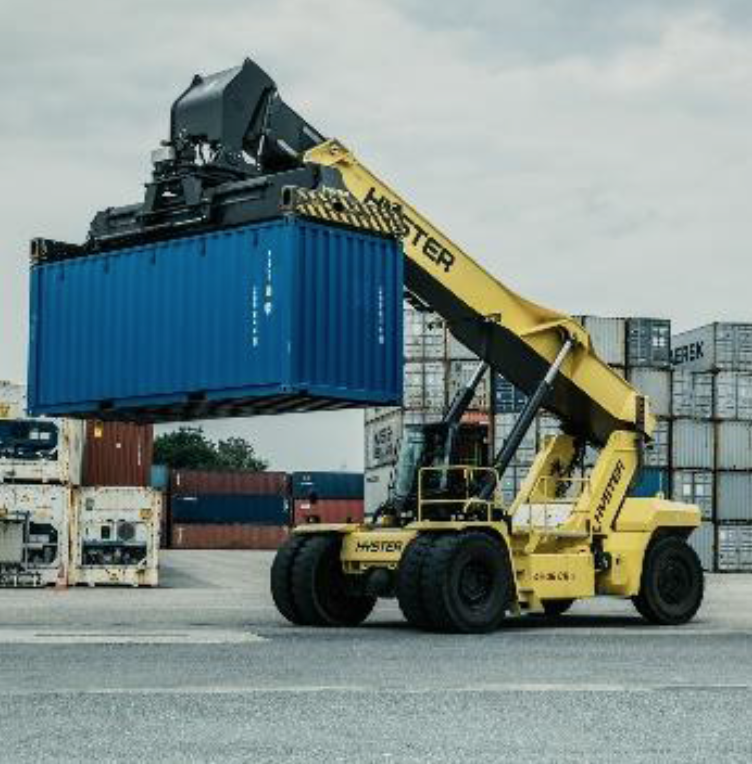
\includegraphics[width=0.7\linewidth]{images/PAS_stacker.png}
\caption{Photo d'un reach-stacker portant un conteneur.}
\label{fig:pas_satellite}
\end{figure}


%Image pour vocabulaire



\section{Présentation du problème et quelques solutions}

\textbf{Objectif : trouver une configuration (une géométrie et une répartition des clients dans cette géométrie) pour minimiser une fonction coût.} \\

\noindent
{\bf Idée :} \\
- la représentation de la hauteur des piles n'a pas d'impact dans le problème car le remplissage et le vidage se font de manière automatique par blocs (qui correspond à une travée) 
avec une catégorie de conteneurs (même client et mêmes dimensions). De plus la gestion des blocs est gérée par leur système informatique (TOS). Nous pouvons donc uniquement optimiser le plan des emplacements dans la cour de stockage.
Nous pouvons donc nous ramener à un problème de surface au sol en considérant chaque travée indépendamment. 
Nous passons d'un problème en 3D où il aurait fallu considérer les conteneurs à un problème en 2D de répartition des travées dans le port. \\

\noindent
{\bf Problématique :} répartir les (définir si le nombre est connu ou pas ?) travées de manière optimale (en ayant des contraintes sur des largeurs maximales de travées) sur la surface du port en minimisant une fonction coût. Il est important de considérer la largeur des travées car c'est de l'espace alloué à un client qui peut être immobilisé inutilement si le client ne stocke pas assez de conteneurs. Mais faire uniquement des travées de courtes largeurs est aussi une perte de place car cela multiplie les allées de circulation. Il faut aussi vérifier que le plan permette de stocker plus de conteneurs ($5000$ conteneurs) car c'est nécessaire à certaines périodes même si notre configuration n'optimise pas ce cas de figure. \\


\subsection{Petit état de l'art ???}
Plusieurs travaux scientifiques portent sur des optimisations du stockage de conteneurs dans la cour de stockage des terminaux portuaires.

% https://www.researchgate.net/publication/294799315_Container_stacking_problem_a_survey



Solution 1 : \\
- le problème revient à mailler la surface disponible dans le port avec des briques de taille 20*8pieds (petit conteneur), puis à repartir sur cette surface les travées (de tailles indiquées sur le plan) et les allées de circulations pour minimiser la distance. La meilleure configuration sera celle qui minimise une fonction coût qui doit être définie.  \\


Solution 2 : \\
- s'inspirer des problèmes de stationnement des avions dans les aéroports, voir par exemple les deux références suivantes : "Optimisation du trafic au sol sur les grands aéroports" de Gotteland et "Optimisation des séquences de pistes et des mouvements au sol sur les grands aéroports" de Deau. \\

Solution : \\
- optimisation de forme, level set (Yannick)

Solution 3 : \\
- combinatoire\\

Solution 4 : \\
- heuristique \\

Solution 5 : \\
- problème de répartition d'objets 2D sur une surface, voir la thèse qui traite les cas 2D et 3D "Méthode générique pour l’optimisation d’agencement géométrique et fonctionnel" de Jacquenot

Solution 6: \\ 
???
-voir référence en 3D "The optimal determination of the space requirement and the number of transfer cranes for import containers" écrit par Kap Hwan Kim and Hon Bae Kim.


\section{Comparaison de plusieurs agencements géométriques de la cour de stockage}

\subsection{Intuition sur le plan des emplacements}

- La zone de "chargement/déchargement camion" doit être au barycentre (pondéré ?) du stockage. S'il y a plusieurs zones de "chargement/déchargement camion", barycentre de sa zone. Mais cette information ne tient pas compte de la contrainte de sécurité pour éviter les nombreux croisements entre camions et reach-stackers. \\

- Avec l'hypothèse que chaque conteneur vide arrive par bateau et part en camion, on connaît exactement son trajet (pas d'incertitude sur le terminal bateau car il ARRIVE par ce terminal). D'où l'idée de couper la zone en deux selon une symétrie à déterminer et d'optimiser le stockage de chaque zone indépendamment. Chaque zone gérerait les conteneurs vides arrivés par son propre terminal bateau. Cela permettrait de toujours stocker les conteneurs "entre" le terminal et la zone de "chargement/déchargement camion". \\


\subsection{Définition de la fonction coût}

Pour comparer différentes configurations, il y a besoin de définir une fonction coût qui évalue leurs performances. \\ Rappel: une configuration est une géométrie et une répartition des clients dans cette géométrie. \\


La fonction coût cherche à évaluer les coûts moyens liés aux emplacements des $4500$ EVP présent en moyenne dans le port. Cette fonction coût tient compte des déplacements entrée-sortie en fonction de la fréquence de déplacement des conteneur qui peut dépendre de chaque client.\\


- Il faut prendre en compte toutes les distances parcourues par les conteneurs, c'est-à-dire depuis leurs arrivées au port et jusqu'à leurs sorties. Comme nous avons peu d'informations sur le pourcentage de conteneurs entrant pour chacun des deux portiques bateau, ???\\
- Pour être considérée comme allée de circulation, celle-ci doit faire 15m de large minimum, \\
- Il faut atteindre la travée par sa largeur (aller chercher le conteneur du c\^oté où c'est possible), \\
- Par catégorie (client+dimensions) ou par client, nous définissons un \textbf{poids} qui est calculé est fonction de la fréquence des mouvements et un \textbf{volume} qui représente un nombre de conteneurs stockés dans le port en moyenne. Cela permet de déterminer la répartition des clients dans une géométrie fixée. Ex: un client stockant peu de conteneurs mais faisant beaucoup de mouvements (entrée ou sortie de conteneurs) devra avoir une courte travée et être à courte distance; un client stockant un gros volume et faisant beaucoup de mouvements pourra avoir des travées plus larges (ou de nombreuses petites travées) et être à courte distance; un client faisant peu de mouvements pourra être stocké plus loin. \\ % formule fréquence


somme sur les travées de (  poids*(dist(portique bateau/travée)+dist(travée/chargement camion))*largeur(travée)  ) \\


\paragraph{Notations}
\begin{table}[h!]
\centering
 \begin{tabular}{|c|c|}
\hline
$t$ & indice de travée \\
$c$ & indice de client \\
$N_t$ & largeur de la travée $t$ \\
& nombre de conteneurs maximum à l'étage 0 dans la travée \\
$V_c$ & nombre "moyen" de conteneurs stoqués sur le port par le client $c$ \\
$V_{tot}$ & nombre total de conteneurs (tous clients confondus) \\
& $\sum_{c} V_c = V_{tot}$ tous les conteneurs appartiennent à un client \\
$x_{t,c}$ & nombre d'emplacements utilisés par le client $c$ dans la travée $t$ \\
 & on est en 2D donc nombre de conteneurs = 5*nombre d'emplacements = $5x_{t,c}$ \\
 & $x_{t,c}*x_{t,c'}=0$ 2 clients différents ne sont pas dans la même travée \\
$d_t$ & dist(portique bateau/travée)+dist(travée/chargement camion \\
$\mu_c$ & poids représentant la fréquence de mvt du client $c$ \\
 & mvt = entrée ou sortie de conteneurs \\
\hline
\end{tabular}
\end{table}

\paragraph{fonction coût}
$\sum_t \sum_c (d_t * \mu_c * x_{t,c})$


\paragraph{Contraintes de la configuration (indépendant de la fonction coût)}
\begin{itemize}
\item tous les conteneurs sont répartis parmi les clients :
$\sum_{c} V_c = V_{tot}$ 
\item dans chaque travée, il y n'y a pas plus d'emplacements utilisés que d'emplacements disponibles :
$\sum_c 0\le x_{t,c} \le N_t \quad \forall t$ 
\item deux clients différents ne peuvent pas être dans la même travée :
$x_{t,c}*x_{t,c'}=0 \quad \forall t \quad \forall c \neq c' $
\item il y a un nombre limité de travées très larges :
$Card(N_t | N_t\ge 6) \le 30$
\item une travée ne peut pas être de taille illimitée :
$1 \le N_t \le 15$
\end{itemize}

\subsection{Cas test ???}
En moyenne $3000$ conteneurs vides (toutes tailles confondues) sont stockés dans la cour de stockage du PAS. Pour simplifier, nous considérons  $V_tot=4500$ EVP. \\

Pour définir un nombre de client et les poids ($\mu_c$)  représentant la fréquence de mouvement des clients, nous avons exploités les donnés que le PAS a mis à notre disposition sur les mouvements des mois de septembre et octobre 2018. 
$
\mu_c = \frac{\sum_{} mvt du client c}{mvt totaux} 
$



\paragraph{Pour aller plus loin : création de plan d'emplacements avec un algorithme de type "snake"} % algorithme rampant

Dans ce paragraphe est introduite une idée d'algorithme pour créer un grand nombre de plans d'emplacements sur lesquels la fonction peut être appliquée pour choisir le meilleur. \\

Les algorithmes de type "snake" consiste à créer des chemins à partir d'un point de départ (l'embarcadère bateau dans notre cas). % biblio ???

Initialisation : \\
- discrétiser le plan du port autonome avec des mailles de la taille du plus petit conteneur, chaque maille est appelée "pixel" dans la suite. On note $(dx,dy)$ la taille d'une maille, \\
- chaque pixel est : soit une allée de circulation ($a$), soit un emplacement ($e$), \\
- définir un nombre minimum d'emplacements ($N_e=4500$), \\

Algorithme :
\begin{itemize}
    \item initialiser tous les pixels à $e$ (ce sont des emplacements), et initialiser la position du snake sur l'embarcadère $(x_0,y_0) = (x_{bateau}, y_{bateau})$,
    \item  boucle tant que $#e>N_e$ (le nombre d'emplacements est suffisamment grand): \\
 1) le serpent se déplace à la position $(x_{i+1},y_{i+1})$ avec 
 \begin{eqnarray}
x_{i+1} = \left\{\begin{array}{l}
x_i, \\
x_i + dx,\\
x_i + dx, \\
\end{array}\right. \qquad
y_{i+1} = \left\{\begin{array}{l}
y_i, \\
y_i + dy,\\
y_i + dy. \\
\end{array}\right.
\nonumber
\end{eqnarray}
 
2) boucle en forme d'escargot autour de $(x_{i+1},y_{i+1})$ pour labéliser en allée $a$ tous les pixels dont la distance avec $(x_{i+1},y_{i+1})$ est inférieure à $15+\sqrt{(dx^2+dy^2)}/2$m ($\sqrt{(dx^2+dy^2)}/2$ car la distance est calculée avec le centre de la maille alors que le reach-stacker ne doit pas taper dans les coins du conteneur), \\
3) mise-à-jour du nombre d'emplacements disponible

\item vérifier que le plan ainsi obtenu respecte les contraintes (dont celle que le camion appartienne à un chemin) et lui appliquer la fonction coût.
\end{itemize}


\section{Intuition sur FIFO}

Une des hypothèses qui oblige à contrainte fortement la géométrie du stockage est liée au \textit{First In, First Out}. En effet, cela suppose d'avoir accès aux conteneurs par les deux côtés opposés de la travée et cela impose d'optimiser la longueur d'une travée en fonction du volume et de la fréquence de mouvements de chaque client. Car le remplissage d'un bloc doit se faire d'un côté et le vidage de l'autre pour avoir accès à la pile la plus vieille de cette travée. Cette hypothèse (FIFO) est faite car la facturation au client dépend de la durée depuis laquelle chaque conteneur est stocké dans le port. Une gestion \textit{Last IN, First Out (LIFO)} du stockage permettrait de réduire énormément les surfaces allouées aux allées de circulations et permettrait d'aller chercher le plus souvent les conteneurs qui demandent le moins de distance globale (distance d'entrée dans le port et de sortie). Une idée naïve évoquée en équipe pendant cette semaine serait d'avoir deux stratégies différentes pour le stockage et la facturation. \textbf{Il s'agit de facturer en FIFO mais de gérer le stockage en LIFO}. 



\section{old: Lancement du travail}

Mardi 13 nov. 2018: lancement du travail le matin puis visite du site à 14h. \\

Objectifs: \\
- on cherche à minimiser la distance parcourue par le container vide entre son arrivée bar barge et son lieu de stockage, et de son stockage à sa sortie par camion, \\
- les variables à utiliser sont l'emplacement de la zone de chargement et déchargement des camions, la géométrie de la zone de stockage, et l'emplacement du container dans cette zone, \\
- les contraintes sont pour la géométrie de respecter les 15m de circulation des reach-stackers, de regrouper les containers par client, ne pas dépasser 6 blocs superposés sur 2 rangées (en pratique 5 rangées car elles sont atteintes depuis 2 allées de circulation). \\

Pour cela, on va se placer dans le cas statique (l'arrivée des conteneurs est déterministe), ce qui consiste à déterminer un plan de stockage optimal .
Pour minimiser la fonction coût, il faut connaître la porte de sortie du container (camion ou quel portique bateau), ce qui n'est pas le cas aujourd'hui.
Pour la SEME, nous allons simplifier le problème en supposant que l'on a qu'une unique sortie, par exemple celle du camion vu que c'est celle sur laquelle on peut jouer. 

Il faut définir mathématiquement la fonction coût et les contraintes associées, par exemple en s'appuyant sur la thèse fournie par Myriam ("Algorithmes d'optimisation pour la résolution du problème de stockage de conteneurs dans un terminal portuaire" écrite par Ndèye Fatma Ndiaye). \\

Dans un autre temps, on essaiera d'exploiter les données des 2 derniers mois fournies par le PAS pour faire une analyse exploratoire. Il faut vérifier d'abord que toutes les données nécessaires soient présentes et exploitables.



\subsection{old: Hypothèses et formulation du problème}

Inspiré de la thèse "Algorithmes d'optimisation pour la résolution du problème de stockage de conteneurs dans un terminal portuaire" écrite par Ndèye Fatma Ndiaye. \\


Dans les méthodes de résolution que nous proposons, nous considérons les quatre hypothèses suivantes. \\
1) On tient compte des différences de taille entre les conteneurs, et on stocke dans chaque pile uniquement des conteneurs de mêmes dimensions. \\
2) Des conteneurs sont de même catégorie s'ils ont les mêmes dimensions et s'ils appartiennent à un même client. \\
3) On suppose que les conteneurs sont numérotés suivant leurs ordres d'arrivée et de déchargement. \\
4) On considère que les piles sont référencées :
La codification des emplacements est composé d'un code alphanumérique sous la forme A(N).NN.NN / N
où A représente une lettre, N représente un chiffre et les () un caractère non obligatoire. Ce code est complété par un niveau (de 0 à 5, 0 étant le niveau du sol). Exemple I7.02.01/4 = bloc.travée.pile/étage



\begin{table}[h!]
\centering
 \begin{tabular}{|c|c|}
\hline
$N$ & nombre total de conteneurs \\
$K$ & conteneur (numéro global du conteneur), $1\ge K \ge N$ \\
$R_K$ & dimension du conteneur K \\
$A_K$ & date d'arrivée du conteneur K \\
$C_K$ & client à qui appartient le conteneur K \\
\hline
$b,t$ & bloc.travée (pour connaître la distance entre entrée/sortie et la travée) \\
$p,e$ & pile.étage (pour connaître où va être stocker le conteneur si en entrée \\
& ou permet de connaître le coût de recherche du conteneur en sortie) \\
\hline
\end{tabular}
\end{table}

$b\in\{A1,...,K3\} = [1,B] = \cal{B}$ \\
$t\in[1,T_b] = \cal{T}_b$ \\
$p\in[1,P_{b,t}] = \cal{P}_{b,t}$ \\
$e\in[0,4] = \cal{E}$ \\


Remarque: si le conteneur est en entrée dans le port, i est donné par l'ordre de remplissage pré-défini d'une travée. \\


$x^K_{b,t,p,e} = 0$ ou $1$ si le conteneur K est à l'emplacement (b,t,p,e) \\
$z^K_{b,t,p,e} = $ coût pour récupérer K dans la pile p à l'étage e



\paragraph{Contraintes:}

\begin{itemize}

\item Chaque conteneur est à un unique emplacement
$$
\sum_{b\in\cal{B}} \sum_{t\in\cal{T}_b} \sum_{p\in\cal{P}_{b,t}} \sum_{e\in\cal{E}}
x^K_{b,t,p,e} = 1 \quad \forall K\in[1,N]
$$ 
\item Chaque emplacement contient maximum un conteneur
$$
\sum_{K\in[1,N]} x^K_{b,t,p,e} \le 1 \quad \forall
$$
\item Les conteneurs d'un même client doivent être dans une même zone ?

\item Chaque travée doit être rempli d'une manière spécifique
\end{itemize}






\end{document}
